\chapter{ОБЗОР АНАЛОГОВ}
    Как уже было отмечено ранее, 3D-сканеры находят применение во множестве областей и решают самые разные задачи. Поэтому на данный момент уже есть готовые устройства, позволяющие производить сканирование, и реализовано несколько методов сканирования, каждый из которых требует разные компоненты и ресурсы. Рассмотрим существующие аналоги таких устройств и соответствующие им методы. Ограничим выбор 3D-сканерами распространяющиеся по open-source модели, поскольку в нашем проекте важна низкая стоимость модуля.
    
    Определим критерии для сравнения устройств:

    \cbox{Описать в каких единицах бывают параметры}
    
    \underline{\textit{Точность}} --- насколько результаты измерения отклоняются от реальных. Один из наиболее важных параметров сканеров. В зависимости от метода колеблется от единиц миллиметров до микрометров.
    
    \underline{\textit{Скорость}} --- насколько быстро производятся вычисления. Многие задачи требуют расчётов в реальном времени и этот критерий является критическим. Как правило Высокая скорость обработки сказывается на точности алгоритма или ограничивает применимость системы (универсальность), поскольку использует специфичные упрощения и аппроксимации.
    
    \underline{\textit{Диапазон измерений}} --- диапазон расстояний (глубины) на которую рассчитано устройство для обеспечения заданной точности. Как правило определяется физическими ограничениями метода и конструкцией. Например размеры матрицы камеры и угол обзора задают верхний порог измерений, а для методов основанных на регистрации импульсов света существует нижний предел измерений обусловленный высокой скоростью света.
    
    \underline{\textit{Габариты}} --- в зависимости от используемой технологии получаются различные габариты и конфигурации. В настоящее время существуют ручные сканеры довольно малых размеров, но также есть и “настольные”, более габаритные устройства.

    \paragraph{Мобильные приложения}
        В настоящее время 3D-технологии довольно распространены, поэтому существуют приложения на смартфон (например, Sony 3D Creator), которые позволяют проводить сканирование любому человеку при наличии девайса поддерживающего необходимые технологии. Такие приложения как правило распространяются бесплатно, что делает её денежно самой выгодной (не считая стоимости смартфона).

        \begin{figure}[H]
            \centering
            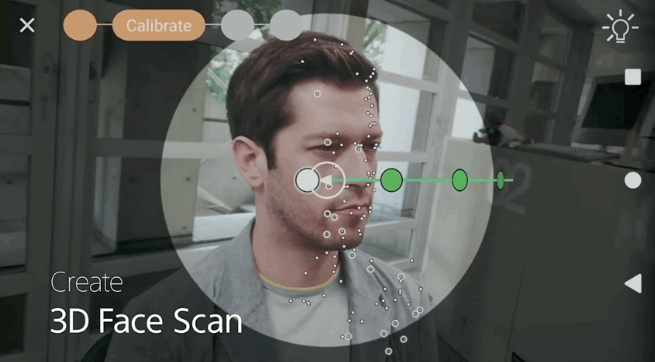
\includegraphics[width=0.5\linewidth]{sony3d}\label{pic:sony3d}
            \caption{Окно приложения Sony 3D creator}
        \end{figure}

        Эти приложения используют метод фотограмметрии для расчётов. Суть данного метода заключается в том, что, имея несколько изображений одного объекта с разных точек обзора, можно сопоставить особые точки (features) этих изображений после чего восстановить модель объекта по каждому пикселю снимков\cite{Guzhov}.

        Метод фотограмметрии, стереоскопия в частности, как правило имеет сравнительно низкую точность, но высокую скорость сканирования. Особенно низкая точность свойственна мобильным приложениям в виду ограниченных вычислительных ресурсов и качества используемых камер. Измерять таким методом можно объекты на расстоянии порядка метра от точки обзора. Габариты и стоимость ограничены используемым смартфоном, однако этот же метод можно использовать с несколькими фиксированными камерами.

        \begin{table}[H]
            \centering
            \caption{Характеристики приложения Sony 3D creator}\label{table:sony3d}
            \begin{tabular}{|l|l|}\hline
                Метод&Фотограмметрия\textbackslash{}стереозрение\\ \hline
                Диапазон&$\approx 1$ м\\ \hline
                Скорость&По завершению съёмки\\ \hline
                Точность&$\approx 1$ мм\\ \hline
                Габариты&Корпус смартфона\\ \hline
                Стоимость&Бесплатно (стоимость смартфона)\\ \hline
            \end{tabular}
        \end{table}

    \paragraph{BQ Ciclop DIY 3D Scanner}
        Это сканер с открытым исходным кодом, предоставляет доступ к 3D-моделям для самостоятельной печати. Представляет из себя поворотную платформу с закреплёнными к ней веб-камере и двумя лазерными модулями. Данное устройство использует метод лазерной триангуляции для расчёта координат в сцене.

        \begin{figure}[H]
            \centering
            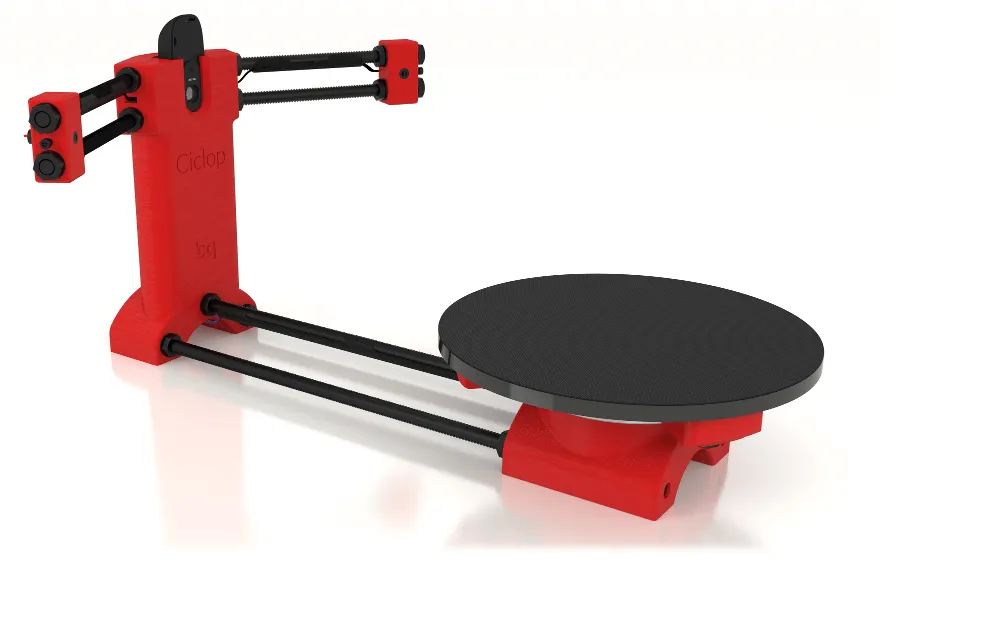
\includegraphics[width=0.5\linewidth]{ciclop}\label{pic:ciclop}
            \caption{Сканер BQ Ciclop}
        \end{figure}

        Суть этого метода в том, что лазер излучает на исследуемую поверхность, которую снимает камера. Камера и лазер при этом должны находиться под углом друг к другу. Таким образом проекция лазера, видимая в кадре, искажается согласно форме исследуемой поверхности. Зная угол и расстояние между камерой и лазером, а так же фокусное расстояние, можно рассчитать координаты засвеченных точек используя отклонение проекции в кадре, так как эти величины формируют подобные треугольники с одной неизвестной величиной -- координатой точки.

        Данный метод, как правило, обладает высокой точностью. В дорогих сканерах (например, Faro ScanArm) точность может быть в пределах микрометров. Но сканирование этим методом может занять некоторое время, т.к. возможно исследовать только один "профиль" сцены за кадр. Таким образом необходимо провести лазером от одного конца сцены до другого, при этом плотность облака напрямую зависит от частоты кадров камеры и скорости движения вдоль сцены.

        Недостатками этого аналога являются его конструкция с поворотным столиком, которую невозможно внедрить в систему. Также нельзя использовать его код, т.к. он написан с учётом конструкции сканера.

        \begin{table}[H]
            \centering
            \caption{Характеристики сканера BQ Ciclop 3D Scanner}\label{table:ciclop}
            \begin{tabular}{|l|l|}\hline
            Метод&Лазерная триангуляция\\ \hline
            Диапазон&$\O250 \times 205$ мм\\ \hline
            Скорость&2-8 минут на оборот\\ \hline
            Точность&$\approx 0.5$ мм\\ \hline
            Габариты&$ 500 \times 300 \times 230 $ мм\\ \hline
            Стоимость&6 000 р.\\ \hline
            \end{tabular}
        \end{table}

    \paragraph{hesamh DIY 3D Scanner}
        Данный аналог это открытый проект за авторством пользователя hesamh основанный на методе структурированного света. Сканер собран из старого проектора и двух веб-камер, закреплённых на деревянном основании. Для этого проекта в открытом доступе находится инструкция для самостоятельной сборке и он использует свободное программное обеспечение 3DUNDERWORLD для обработки данных.

        \begin{figure}[!ht]
            \centering
            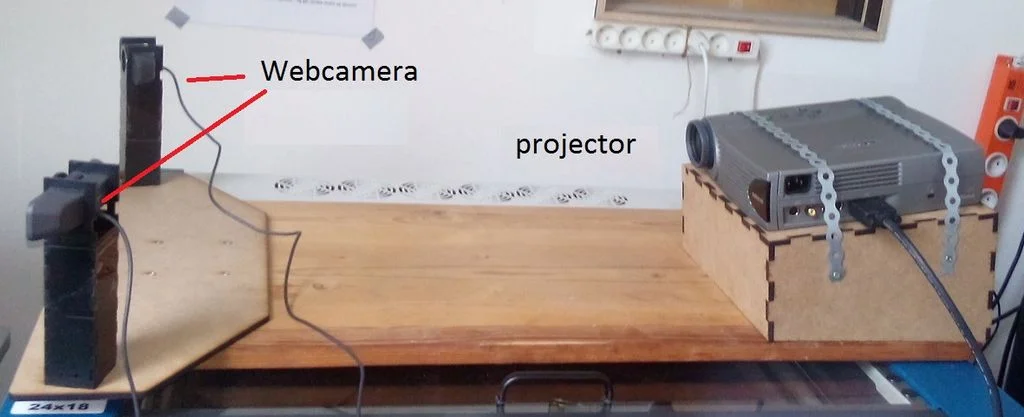
\includegraphics[width=0.5\linewidth]{hesamh}\label{pic:hesamh}
            \caption{Сканер hesamh}
        \end{figure}
        
        Метод структурированного света похож на лазерную триангуляцию (триангуляция с проекцией линией является частным случаем), но использует специальный рисунок (паттерн), как правило чередующихся чёрных и белых полос. Этот рисунок также проецируется на объект, с помощью проектора, и искажения рисунка соответствуют форме объекта. Данный метод обладает в общем случае такой же точностью как метод лазерной триангуляции, но позволяет получить больше информации из одного кадра. Однако при этом необходим более сложный алгоритм для обработки данных с камеры. Другим существенным недостатком этого метода является необходимость использовать проектор, что значительно увеличивает его габариты и стоимость по сравнению с другими методами.
        
        \begin{table}[H]
            \centering
            \caption{Характеристики сканера от hesamh}\label{table:hesamh}
            \begin{tabular}{|l|l|}\hline
            Метод&Структурированный свет\\ \hline
            Диапазон&до 2 м от камеры\\ \hline
            Скорость&-\\ \hline
            Точность&$\approx 0.5$ мм\\ \hline
            Габариты&$ 1000 \times 500 \times 300 $ мм\\ \hline
            Стоимость&$\sim 10 000\text{ р.}$\\ \hline
            \end{tabular}
        \end{table}